\chapter{A New Approach}

In this chapter, we will present a noval approach for rendering a scene with dynamic light source efficiently. This method is based d on the standard GPU-based photon mapping rendering system, using an augmented kd-tree data structure and localized updating algorithm for rendering.  

In the first 2 sections of this chapter, We will have an overview on our approach and comprehensive description of the data structure that we use and related algorithms. Then we will look at some of the GPU implementation details. 

\section{Overview} 

As described in chapter 2, we build a gloabl kd-tree as the photon map for irradiance estimation. However, the global photon map is rebuilt from scratch every frame, this process is time consumings due to the complexity of kd-tree building algorigthm on GPUs and can be avoided. 

Instead of building a global kd-tree for photons, we re-use the same kd-tree for the geometry objects(triangles) which is static and associate the geometry and the photons data for efficient KNN search and update for dynamic scene. 

For each frame, the photons are shot from the light source and stored in an array, then we build the kd-tree for the geometry objects if it is required, for the scenes that don't include animated objects we will skip this process. Given the photons data in the scene and the built kd-tree for geometry, we build our data structure, compress the memory bind it to the texture memory for a better memory accessing performance. In rendering phase, instead of using photon map for radiance estimation, we use the kd-tree and our photon queue perform KNN search. Further details of the data structure will be presented in the following section. 

The update process of photons queue is straightforward. It depends on the photon data from the previouse frames. Here we keep track of all the photons data of a range of frames with a pair of indices, the indices can be updated and maintained efficiently. Furthur  details will be presented in following section.  

\section{Data Structure And Algorithm} 

\subsection{Data Structure}

\begin{figure}[htp] 
    \centering 
    \fbox{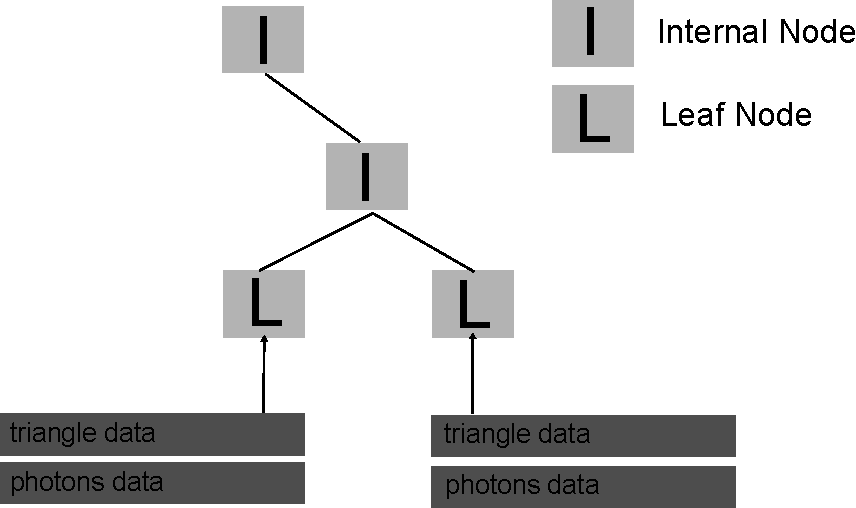
\includegraphics{kd_leaf_photons.pdf}}
    \renewcommand{\thefigure}{\thechapter.\arabic{figure}}
    \caption[]{Radiant flux from a point light source is passing through the spheres around the light.}
    \label{fig:kd_leaf_photons} 
\end{figure}  

As shown in figure \ref{fig:kd_leaf_photons}, in addition to the triangle data, the photons data in the scene is also logically associated with the leaf nodes of the kd-tree. 

\begin{figure}[htp] 
    \centering 
    \fbox{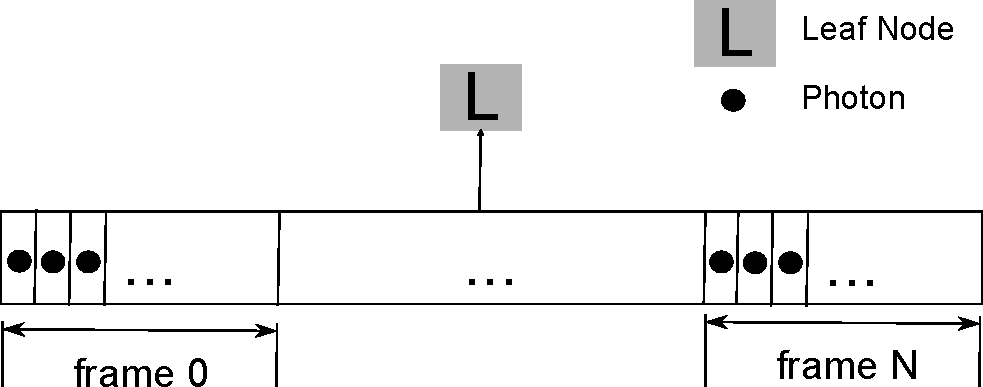
\includegraphics{kd_leaf_photons_2.pdf}}
    \renewcommand{\thefigure}{\thechapter.\arabic{figure}}
    \caption[]{Radiant flux from a point light source is passing through the spheres around the light.}
    \label{fig:kd_leaf_photons_2} 
\end{figure}  




\subsection{Construction} 


\subsection{Update} 


\subsection{Rendering} 

\section{Implementation Details} 
